%=================================================================
% CSE 4345 — Big Data Analytics
% Week 2, Part 2: Seminal Research & Case Study
% Department of CSE, Premier University
%
% SEMINAL PAPER:
%   Halevy, Rajaraman & Ordille (2006) — Data Integration: The Teenage Years
%   VLDB 2006 (cited >1,500 times)
%
% CASE STUDY:
%   HL7 FHIR in US Healthcare — Federated ETL Integration at National Scale
%=================================================================

\documentclass[aspectratio=169,10pt]{beamer}

%---------- Packages ----------
\usepackage[utf8]{inputenc}
\usepackage[T1]{fontenc}
\usepackage{booktabs}
\usepackage{xcolor}
\usepackage{tikz}
\usetikzlibrary{shapes.geometric, positioning, arrows.meta, decorations.pathreplacing}
\usepackage{amsmath}
\usepackage{graphicx}
\usepackage{multicol}
\usepackage{enumerate}
\usepackage{array}

%---------- Theme ----------
\usetheme{Madrid}

%---------- Premier University Color Identity ----------
\definecolor{PUNavy}{RGB}{10,36,99}
\definecolor{PUGold}{RGB}{197,151,37}
\definecolor{PULightBlue}{RGB}{210,228,255}
\definecolor{PUTeal}{RGB}{0,100,100}
\definecolor{PUGray}{RGB}{90,90,90}
\definecolor{PURed}{RGB}{160,30,30}
\definecolor{PUGreen}{RGB}{30,120,60}
\definecolor{PUPurple}{RGB}{90,30,120}
\definecolor{PUOrange}{RGB}{190,90,20}

\setbeamercolor{palette primary}{bg=PUNavy, fg=white}
\setbeamercolor{palette secondary}{bg=PUNavy!85, fg=white}
\setbeamercolor{palette tertiary}{bg=PUNavy!70, fg=white}
\setbeamercolor{palette quaternary}{bg=PUNavy, fg=white}
\setbeamercolor{structure}{fg=PUNavy}
\setbeamercolor{title}{bg=PUNavy, fg=PUGold}
\setbeamercolor{subtitle}{fg=white}
\setbeamercolor{frametitle}{bg=PUNavy, fg=PUGold}
\setbeamercolor{alerted text}{fg=PUGold!85!black}
\setbeamercolor{block title}{bg=PUNavy, fg=white}
\setbeamercolor{block body}{bg=PULightBlue!45}
\setbeamercolor{block title alerted}{bg=PUGold!80!black, fg=white}
\setbeamercolor{block body alerted}{bg=PUGold!12}
\setbeamercolor{block title example}{bg=PUTeal, fg=white}
\setbeamercolor{block body example}{bg=PUTeal!10}
\setbeamercolor{section in toc}{fg=PUNavy}
\setbeamercolor{itemize item}{fg=PUGold!80!black}
\setbeamercolor{itemize subitem}{fg=PUNavy!70}

\setbeamertemplate{navigation symbols}{}
\setbeamertemplate{itemize item}{\scriptsize\raise1.5pt\hbox{\textbullet}}
\setbeamertemplate{itemize subitem}{\scriptsize\raise1pt\hbox{--}}

%---------- Section separator ----------
\AtBeginSection[]{
  \begin{frame}[plain]
    \vfill
    \centering
    \begin{beamercolorbox}[sep=12pt,center,shadow=true,rounded=true]{block title}
      \usebeamerfont{title}\insertsectionhead\par
    \end{beamercolorbox}
    \vfill
  \end{frame}
}

%---------- Helper: citation box ----------
\newenvironment{paperbox}[1]{%
  \setbeamercolor{block title}{bg=PUNavy!90,fg=PUGold}
  \setbeamercolor{block body}{bg=PUNavy!6}
  \begin{block}{#1}}{%
  \end{block}}

%---------- Custom footline ----------
\setbeamertemplate{footline}{
  \leavevmode\hbox{%
    \begin{beamercolorbox}[wd=.333\paperwidth,ht=2.25ex,dp=1ex,center]{palette primary}
      \usebeamerfont{author in head/foot}\insertshortauthor
    \end{beamercolorbox}%
    \begin{beamercolorbox}[wd=.334\paperwidth,ht=2.25ex,dp=1ex,center]{palette secondary}
      \usebeamerfont{title in head/foot}\insertshorttitle
    \end{beamercolorbox}%
    \begin{beamercolorbox}[wd=.333\paperwidth,ht=2.25ex,dp=1ex,right]{palette primary}
      \usebeamerfont{date in head/foot}
      \insertframenumber{} / \inserttotalframenumber\hspace*{2ex}
    \end{beamercolorbox}}%
  \vskip0pt%
}

%---------- Title metadata ----------
\title[CSE 4345 \textbar{} Week 2, Part 2]{CSE 4345: Big Data Analytics}
\subtitle{Week 2, Part 2 \textemdash\ Seminal Research \& Case Study}
\author[Dept.\ of CSE]{Department of Computer Science \& Engineering\\[4pt]
       \small Premier University, Chittagong}
\institute{}
\date{Semester 2026}

%=================================================================
\begin{document}
%=================================================================

%----------------------------------------------------------------
% TITLE SLIDE
%----------------------------------------------------------------
\begin{frame}
  \titlepage
\end{frame}

%----------------------------------------------------------------
% PART 2 OVERVIEW
%----------------------------------------------------------------
\begin{frame}{Part 2 Overview — Week 2}
  \begin{columns}[T]
    \column{0.47\textwidth}
      \begin{block}{Today's Agenda}
        \tableofcontents
      \end{block}

    \column{0.50\textwidth}
      \begin{exampleblock}{Seminal Paper Covered}
        \begin{enumerate}
          \item Halevy, A., Rajaraman, A., \& Ordille, J. (2006).
                \textit{Data Integration: The Teenage Years.}
                VLDB 2006. Seoul, Korea.
        \end{enumerate}
      \end{exampleblock}
      \vspace{6pt}
      \begin{alertblock}{Case Study}
        HL7 FHIR in US Healthcare — national-scale federated health
        data integration under the 21st Century Cures Act (2016).
      \end{alertblock}
      \vspace{4pt}
      \begin{block}{CLO Addressed}
        \textbf{CLO2} — Analyse real-world data integration challenges\\
        \textbf{PLO(b,c)}
      \end{block}
  \end{columns}
\end{frame}

%================================================================
\section{Research Paper — Halevy, Rajaraman \& Ordille (2006)}
%================================================================

%----------------------------------------------------------------
\begin{frame}{Research Landscape: Data Integration Timeline}
  \begin{center}
  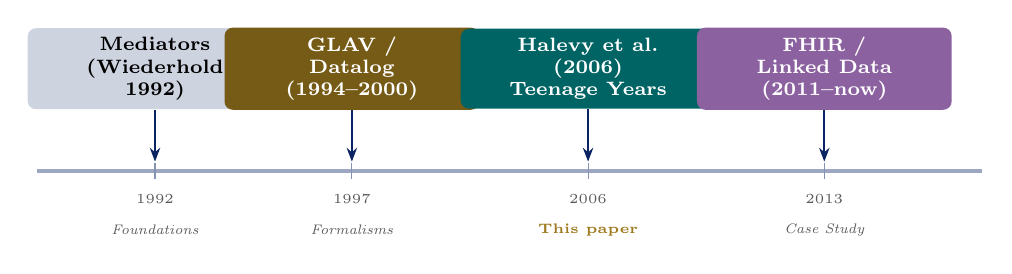
\begin{tikzpicture}[
      nbox/.style={rectangle, rounded corners=3pt, minimum width=3.2cm,
                   minimum height=0.95cm, text width=3.0cm, align=center,
                   font=\scriptsize\bfseries},
      arr/.style={-{Stealth[length=5pt]}, draw=PUNavy, thick}
    ]
    \draw[PUNavy!40, very thick] (0,0) -- (12,0);

    \node[nbox, fill=PUNavy!20]          (med) at (1.5,1.3)
          {Mediators\\(Wiederhold\\1992)};
    \node[nbox, fill=PUGold!60!black, text=white]  (glav) at (4.0,1.3)
          {GLAV /\\Datalog\\(1994--2000)};
    \node[nbox, fill=PUTeal, text=white]            (hro)  at (7.0,1.3)
          {Halevy et al.\\(2006)\\Teenage Years};
    \node[nbox, fill=PUPurple!70, text=white]       (fhir) at (10.0,1.3)
          {FHIR /\\Linked Data\\(2011--now)};

    \foreach \x/\y in {1.5/1992, 4.0/1997, 7.0/2006, 10.0/2013}{
      \draw[PUNavy!50] (\x,0.1) -- (\x,-0.1);
      \node[font=\tiny, text=PUGray] at (\x,-0.35) {\y};
    }

    \draw[arr] (med)  -- (1.5,  0.12);
    \draw[arr] (glav) -- (4.0,  0.12);
    \draw[arr] (hro)  -- (7.0,  0.12);
    \draw[arr] (fhir) -- (10.0, 0.12);

    \node[font=\tiny\itshape, text=PUGray]           at (1.5, -0.75) {Foundations};
    \node[font=\tiny\itshape, text=PUGray]           at (4.0, -0.75) {Formalisms};
    \node[font=\tiny\bfseries, text=PUGold!80!black] at (7.0, -0.75) {This paper};
    \node[font=\tiny\itshape, text=PUGray]           at (10.0,-0.75) {Case Study};
  \end{tikzpicture}
  \end{center}
  \vspace{4pt}
  \begin{alertblock}{Why This Sequence?}
    Wiederhold (1992) introduced mediator architectures $\to$
    the GLAV decade formalised schema mappings $\to$
    Halevy et al.\ (2006) honestly audited what \emph{hadn't} worked and proposed the \textbf{pay-as-you-go} paradigm $\to$
    FHIR / Linked Data put those lessons into production.
    Week 2 builds on all four layers.
  \end{alertblock}
\end{frame}

%----------------------------------------------------------------
\begin{frame}{Halevy et al.\ (2006): Publication Context}
  \begin{columns}[T]
    \column{0.53\textwidth}
      \begin{paperbox}{Full Citation}
        Halevy, A., Rajaraman, A., \& Ordille, J. (2006).
        \textbf{Data Integration: The Teenage Years.}
        In \textit{Proceedings of the 32nd International Conference on
        Very Large Data Bases (VLDB)}, pp.~9--16. Seoul, Korea.\\[5pt]
        \textbf{Venue:} VLDB — Rank A* (CORE), top-tier DB venue\\
        \textbf{Cited by:} $>$1{,}600 (Google Scholar, 2024)\\
        \textbf{Authors:} Alon Halevy (Google), Anand Rajaraman (Amazon A9),
        Jayant Ordille (Yahoo! Research)
      \end{paperbox}
      \vspace{5pt}
      \begin{exampleblock}{Historical Moment}
        By 2006, data integration research was $\approx$15 years old
        (``teenage'').  Three industry heavyweights wrote an honest
        retrospective — celebrating progress, naming failures,
        and redirecting the field.
      \end{exampleblock}

    \column{0.44\textwidth}
      \begin{block}{The Core Question}
        \begin{center}
        \large\color{PUNavy}
        ``\textit{Why, after 15 years of\\research, do enterprises\\
        still struggle to integrate\\their data?}''
        \end{center}
      \end{block}
      \vspace{8pt}
      \begin{alertblock}{The Answer (in one sentence)}
        Because perfect schema mappings require
        \textbf{semantic understanding} that cannot be automated
        — so the field must shift from \emph{completeness}
        to \emph{incremental, probabilistic integration}.
      \end{alertblock}
  \end{columns}
\end{frame}

%----------------------------------------------------------------
\begin{frame}{Technical Contribution 1 — The Integration Stack}
  \begin{columns}[T]
    \column{0.50\textwidth}
      \begin{block}{The Classic Mediator–Wrapper Architecture}
        \begin{itemize}
          \item \textbf{Wrappers} expose each data source through a
                uniform query interface (relational, XML, or object)
          \item \textbf{Mediator} holds a \textbf{global schema} and
                rewrites queries into sub-queries against wrappers
          \item \textbf{Schema mappings} (the hard part): declarative
                rules that translate between source and global schemas
          \item The dominant formalism: \textbf{GLAV} (Global-Local-As-View)
                — sources defined as views over the global schema
                \emph{and} vice versa; allows bidirectional query rewriting
        \end{itemize}
      \end{block}
      \vspace{5pt}
      \begin{alertblock}{The Semantic Gap Problem}
        Even with perfect GLAV mappings, the \emph{meaning} of
        \texttt{customer\_id} in the Sales DB $\neq$
        \texttt{cust\_no} in the CRM — no formal system can resolve
        this without \textbf{domain expertise}.
      \end{alertblock}

    \column{0.47\textwidth}
      \begin{center}
      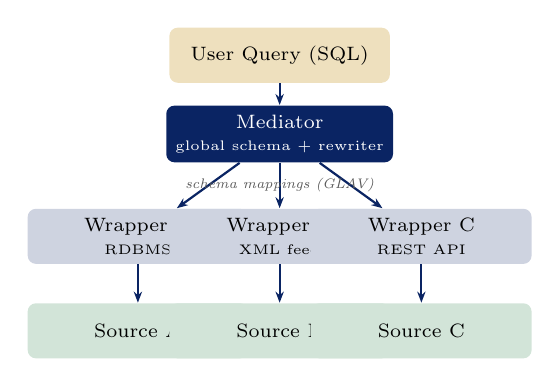
\begin{tikzpicture}[
          box/.style={rectangle, rounded corners=3pt, minimum width=2.8cm,
                      minimum height=0.7cm, align=center, font=\scriptsize},
          arr/.style={-{Stealth[length=4pt]}, draw=PUNavy, thick}
        ]
        \node[box, fill=PUGold!30]  (q)   at (0, 3.8) {User Query (SQL)};
        \node[box, fill=PUNavy, text=white] (med) at (0, 2.8)
              {Mediator\\{\tiny global schema + rewriter}};
        \node[box, fill=PUNavy!20]  (wa)  at (-1.8, 1.5) {Wrapper A\\{\tiny RDBMS}};
        \node[box, fill=PUNavy!20]  (wb)  at (0,    1.5) {Wrapper B\\{\tiny XML feed}};
        \node[box, fill=PUNavy!20]  (wc)  at (1.8,  1.5) {Wrapper C\\{\tiny REST API}};
        \node[box, fill=PUGreen!20] (sa)  at (-1.8, 0.3) {Source A};
        \node[box, fill=PUGreen!20] (sb)  at (0,    0.3) {Source B};
        \node[box, fill=PUGreen!20] (sc)  at (1.8,  0.3) {Source C};

        \draw[arr] (q)  -- (med);
        \draw[arr] (med)-- (wa);
        \draw[arr] (med)-- (wb);
        \draw[arr] (med)-- (wc);
        \draw[arr] (wa) -- (sa);
        \draw[arr] (wb) -- (sb);
        \draw[arr] (wc) -- (sc);

        \node[font=\tiny\itshape, text=PUGray] at (0, 2.15)
              {schema mappings (GLAV)};
      \end{tikzpicture}
      \end{center}
  \end{columns}
\end{frame}

%----------------------------------------------------------------
\begin{frame}{Technical Contribution 2 — Pay-As-You-Go Integration}
  \begin{columns}[T]
    \column{0.52\textwidth}
      \begin{block}{The Paper's Central Proposal}
        Traditional integration demands \textbf{complete, correct schema
        mappings before any query can run}.
        This is the primary reason real projects fail or are abandoned
        after months of schema work.\\[5pt]
        \textbf{Pay-as-you-go (PAYG) integration} (Halevy et al.\ 2006):
        \begin{enumerate}
          \item Start with \emph{imperfect} mappings (even keyword-level)
          \item Return \emph{ranked, uncertain} answers rather than blocking on completeness
          \item Improve mappings \emph{incrementally} as usage reveals gaps
          \item Track \textbf{data provenance} so downstream consumers know source quality
        \end{enumerate}
      \end{block}
      \vspace{5pt}
      \begin{exampleblock}{Analogy (from the paper)}
        Like a teenager's knowledge: incomplete, sometimes wrong, but
        \emph{functional and improving} — better than waiting for
        a perfect adult to arrive.
      \end{exampleblock}

    \column{0.45\textwidth}
      \begin{alertblock}{Why Schema Matching Fails at Scale}
        \begin{itemize}
          \item $n$ schemas $\Rightarrow$ $O(n^2)$ pairwise mappings needed
          \item Each mapping requires \textbf{semantic consensus}
                from domain owners (weeks of meetings)
          \item Sources evolve; mappings \textbf{rot silently}
          \item No enterprise has ever fully mapped $>$50 source schemas
                using the classical approach
        \end{itemize}
      \end{alertblock}
      \vspace{6pt}
      \begin{block}{Dataspace Systems (Halevy et al.\ PODS 2006)}
        A \textbf{dataspace} manages heterogeneous data
        \emph{without} upfront integration — co-existence first,
        mapping second.
        Think: Google's internal data lake before BigQuery APIs.
      \end{block}
  \end{columns}
\end{frame}

%----------------------------------------------------------------
\begin{frame}{Technical Contribution 3 — Semantic Heterogeneity Taxonomy}
  \begin{columns}[T]
    \column{0.50\textwidth}
      \begin{block}{Four Levels of Mismatch (Halevy et al.\ 2006)}
        \renewcommand{\arraystretch}{1.25}
        \begin{tabular}{@{}p{2.0cm}p{4.0cm}@{}}
          \toprule
          \textbf{Level} & \textbf{Example} \\
          \midrule
          Naming     & \texttt{cust\_id} vs.\ \texttt{customer\_no} \\
          Structural  & flat table vs.\ nested JSON \\
          Semantic    & \texttt{revenue} (gross) vs.\ \texttt{revenue} (net) \\
          Temporal    & daily snapshot vs.\ event stream \\
          \bottomrule
        \end{tabular}
      \end{block}
      \vspace{5pt}
      \begin{alertblock}{Key Insight}
        \textbf{Naming and structural} mismatches can be solved by
        schema-matching algorithms (ML-based, 2024: LLMs).
        \textbf{Semantic and temporal} mismatches require \emph{human
        domain knowledge} — no algorithm can determine whether
        ``revenue'' means gross or net.
      \end{alertblock}

    \column{0.47\textwidth}
      \begin{block}{Halevy's Prescription}
        \begin{itemize}
          \item \textbf{Invest in metadata}: every dataset should carry
                a machine-readable description of semantics
                (today: data catalogs — Apache Atlas, DataHub, Alation)
          \item \textbf{Embrace uncertainty}: integration results should
                carry \textbf{confidence scores and provenance lineage}
                (today: dbt lineage, OpenLineage)
          \item \textbf{Domain ownership}: the producing team is the
                only reliable author of semantic documentation
                (today: \textbf{Data Mesh} principle~1)
          \item \textbf{Probabilistic mapping}: use Bayesian schema
                matching rather than deterministic rules
        \end{itemize}
      \end{block}
  \end{columns}
\end{frame}

%----------------------------------------------------------------
\begin{frame}{Impact Today — Halevy et al.\ (2006)}
  \begin{columns}[T]
    \column{0.50\textwidth}
      \begin{block}{Concepts from the Paper Still in Active Use}
        \begin{itemize}
          \item \textbf{Data catalogs} — Apache Atlas, DataHub, Alation
                implement ``dataspace co-existence'' as their core model
          \item \textbf{Schema registry} — Confluent Schema Registry,
                AWS Glue Catalog apply PAYG registration
          \item \textbf{Data lineage} — OpenLineage, dbt implements
                provenance tracking proposed in the paper
          \item \textbf{Data Mesh} — Dehghani (2019) explicitly cites
                Halevy's ``domain ownership'' prescription as an ancestor
          \item \textbf{LLM-based schema matching} — GPT-4 / Gemini
                used as mediators; Halevy himself co-authored work at
                Google on this (2023)
        \end{itemize}
      \end{block}

    \column{0.47\textwidth}
      \begin{exampleblock}{Stanford CS246 / CMU 15-721 Perspective}
        \begin{itemize}
          \item Stanford CS246 covers schema matching as a
                \textbf{set-similarity / embedding} problem (Jaccard +
                word2vec on column names)
          \item CMU 15-721 frames integration as a \textbf{query
                federation} problem: how to push predicates through
                heterogeneous wrappers efficiently
          \item Both courses trace the theoretical lineage directly
                to Halevy et al.\ 2006
        \end{itemize}
      \end{exampleblock}
      \vspace{5pt}
      \begin{alertblock}{CLO2 Connection}
        By analysing \emph{why} classical integration fails,
        students can design systems that avoid the $O(n^2)$
        schema-mapping trap — the \textbf{core CLO2 skill}.
      \end{alertblock}
  \end{columns}
\end{frame}

%================================================================
\section{Case Study — HL7 FHIR: Healthcare Data Integration at Scale}
%================================================================

%----------------------------------------------------------------
\begin{frame}{The Healthcare Data Integration Problem}
  \begin{columns}[T]
    \column{0.52\textwidth}
      \begin{block}{Why Healthcare Data is the Hardest Integration Domain}
        \begin{itemize}
          \item A typical US hospital has \textbf{50–400 distinct systems}:
                EHR (Epic, Cerner), lab (LIMS), radiology (PACS),
                pharmacy (Pyxis), billing (IDX), scheduling, and dozens more
          \item Each system uses \textbf{its own data model and vocabulary}
          \item Patient identity matching across systems:
                no universal patient ID in the US pre-2016
          \item \textbf{HIPAA} (1996) requires strict access control;
                integration cannot expose PHI
          \item Result: clinicians make decisions with \textbf{incomplete data};
                studies estimate 400{,}000 preventable deaths/year in the US
                from medical errors, many information-related
        \end{itemize}
      \end{block}

    \column{0.45\textwidth}
      \begin{center}
      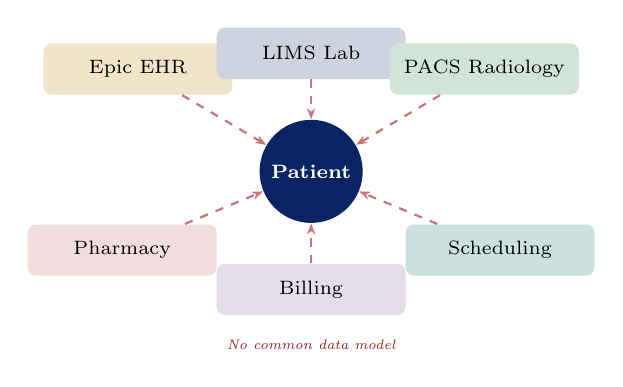
\begin{tikzpicture}[
          sbox/.style={rectangle, rounded corners=3pt, minimum width=2.4cm,
                       minimum height=0.65cm, align=center, font=\scriptsize},
          arr/.style={-{Stealth[length=4pt]}, draw=PURed!60, thick, dashed}
        ]
        % Central patient
        \node[circle, fill=PUNavy, text=white, minimum size=1.1cm,
              font=\scriptsize\bfseries] (pt) at (0, 2.0) {Patient};

        \node[sbox, fill=PUGold!25]    (ehr)  at (-2.2, 3.3) {Epic EHR};
        \node[sbox, fill=PUNavy!20]    (lab)  at (0,    3.5) {LIMS Lab};
        \node[sbox, fill=PUGreen!20]   (rad)  at (2.2,  3.3) {PACS Radiology};
        \node[sbox, fill=PURed!15]     (pharm)at (-2.4, 1.0) {Pharmacy};
        \node[sbox, fill=PUPurple!15]  (bill) at (0,    0.5) {Billing};
        \node[sbox, fill=PUTeal!20]    (sched)at (2.4,  1.0) {Scheduling};

        \foreach \n in {ehr, lab, rad, pharm, bill, sched} {
          \draw[arr] (\n) -- (pt);
        }

        \node[font=\tiny\itshape, text=PURed] at (0, -0.2)
              {No common data model};
      \end{tikzpicture}
      \end{center}
  \end{columns}
\end{frame}

%----------------------------------------------------------------
\begin{frame}[fragile]{HL7 FHIR: The Standard That Changed Healthcare Integration}
  \begin{columns}[T]
    \column{0.52\textwidth}
      \begin{block}{What is HL7 FHIR?}
        \textbf{Health Level Seven} (HL7) International is a standards
        body founded in 1987.
        \textbf{FHIR} (Fast Healthcare Interoperability Resources),
        released as Release 1 in 2014 and R4 in 2019, defines:
        \begin{itemize}
          \item \textbf{Resources}: atomic clinical data objects
                (Patient, Observation, Medication, Encounter — 145+ types)
          \item \textbf{REST API}: \texttt{GET /Patient/\{id\}},
                \texttt{POST /Observation}, standard HTTP verbs
          \item \textbf{SMART on FHIR}: OAuth2-based authorisation
                for third-party app access
          \item \textbf{Terminology binding}: SNOMED CT, LOINC, ICD-10
                as controlled vocabularies (solving semantic heterogeneity!)
        \end{itemize}
      \end{block}

    \column{0.45\textwidth}
      \begin{exampleblock}{Key FHIR Resource (JSON)}
        \scriptsize
        \begin{verbatim}
{
 "resourceType": "Observation",
 "status": "final",
 "code": {
   "coding": [{
     "system": "http://loinc.org",
     "code":   "8480-6",
     "display":"Systolic BP"
   }]
 },
 "valueQuantity": {
   "value":  128,
   "unit":   "mmHg"
 }
}
        \end{verbatim}
      \end{exampleblock}
  \end{columns}
\end{frame}

%----------------------------------------------------------------
\begin{frame}{Case Study: 21st Century Cures Act — National FHIR Mandate}
  \begin{columns}[T]
    \column{0.52\textwidth}
      \begin{block}{The Mandate (US, 2016 / enforced 2021)}
        The \textbf{21st Century Cures Act} required every certified
        EHR vendor in the US to expose patient data via a
        \textbf{FHIR R4 API by April 2021}.
        Penalties for \emph{information blocking}: up to \$1M per violation.
        \begin{itemize}
          \item \textbf{Scale}: $>$350M patients, $>$6{,}000 hospitals,
                $>$900{,}000 clinicians affected
          \item \textbf{Impact}: Apple Health Records, Google Health,
                Amazon HealthLake — all built on this mandate
          \item Every major EHR (Epic, Cerner/Oracle, Allscripts)
                deployed FHIR endpoints in 2020--2021
        \end{itemize}
      \end{block}
      \vspace{4pt}
      \begin{alertblock}{Integration Lesson}
        Regulatory mandate succeeded where 30 years of voluntary
        standards (HL7 v2, HL7 v3, CDA) had failed.
        \textbf{Incentives}, not technology, solved the adoption problem.
      \end{alertblock}

    \column{0.45\textwidth}
      \begin{center}
      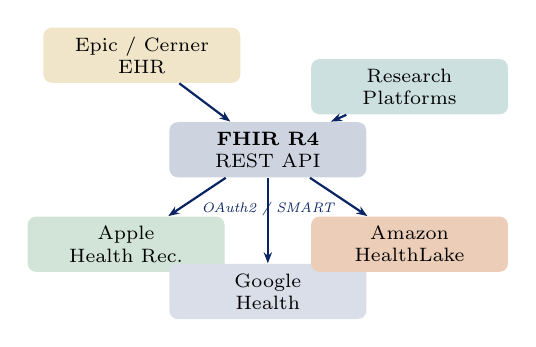
\begin{tikzpicture}[
          pbox/.style={rectangle, rounded corners=3pt, minimum width=2.5cm,
                       minimum height=0.7cm, align=center, font=\scriptsize},
          arr/.style={-{Stealth[length=4pt]}, draw=PUNavy, thick}
        ]
        \node[pbox, fill=PUGold!25]   (ehr)  at (-1.6, 3.2) {Epic / Cerner\\EHR};
        \node[pbox, fill=PUNavy!20]   (fhir) at (0,    2.0) {\textbf{FHIR R4}\\REST API};
        \node[pbox, fill=PUGreen!20]  (apple)at (-1.8, 0.8) {Apple\\Health Rec.};
        \node[pbox, fill=PUNavy!15]   (goog) at (0,    0.2) {Google\\Health};
        \node[pbox, fill=PUOrange!30] (amaz) at (1.8,  0.8) {Amazon\\HealthLake};
        \node[pbox, fill=PUTeal!20]   (res)  at (1.8,  2.8) {Research\\Platforms};

        \draw[arr] (ehr)  -- (fhir);
        \draw[arr] (res)  -- (fhir);
        \draw[arr] (fhir) -- (apple);
        \draw[arr] (fhir) -- (goog);
        \draw[arr] (fhir) -- (amaz);

        \node[font=\tiny\itshape, text=PUNavy] at (0, 1.25)
              {OAuth2 / SMART};
      \end{tikzpicture}
      \end{center}
  \end{columns}
\end{frame}

%----------------------------------------------------------------
\begin{frame}{ETL Architecture Inside a FHIR-Based Health Data Lake}
  \begin{columns}[T]
    \column{0.50\textwidth}
      \begin{block}{Typical Hospital FHIR ETL Pipeline}
        \begin{enumerate}
          \item \textbf{Extract}: Nightly or real-time FHIR API pull
                (\texttt{GET /Patient?\$everything})
                — returns a Bundle of all resources for a patient
          \item \textbf{Transform}: FHIR $\to$ flat Parquet tables
                via Apache Spark + \texttt{fhir.resources} Python library;
                explode nested arrays, resolve LOINC/SNOMED codes
          \item \textbf{Load}: Delta Lake / Apache Iceberg on S3;
                partitioned by \texttt{encounter\_date} and \texttt{patient\_id}
          \item \textbf{Governance}: column-level masking for PHI
                (Azure Purview / AWS Macie), RBAC per department
          \item \textbf{Analytics}: downstream BI (PowerBI),
                cohort queries (Hive/Athena), ML (SageMaker)
        \end{enumerate}
      \end{block}

    \column{0.47\textwidth}
      \begin{exampleblock}{Scale Numbers — Mayo Clinic FHIR Platform}
        \begin{itemize}
          \item \textbf{Source systems}: 35 EHR instances merged
          \item \textbf{FHIR resources}: 4.2 billion stored resources
          \item \textbf{Patients}: 1.3 million active patient records
          \item \textbf{Daily ingestion}: $\approx$12M new FHIR resources/day
          \item \textbf{Query latency}: $<$2 seconds on 5-year patient history
                (via columnar Parquet + predicate pushdown)
          \item \textbf{Schema convergence}: from 35 distinct schemas
                to \textbf{one FHIR R4 global schema}
                — solving the Halevy $O(n^2)$ mapping problem
                through \emph{regulatory standardisation}
        \end{itemize}
      \end{exampleblock}
  \end{columns}
\end{frame}

%----------------------------------------------------------------
\begin{frame}{Lessons Learned \& Discussion Questions}
  \begin{columns}[T]
    \column{0.52\textwidth}
      \begin{block}{Key Lessons from the FHIR Case}
        \begin{enumerate}
          \item \textbf{Canonical data model wins}: all 35 EHR schemas
                converged to FHIR R4 — the ``global schema''
                Halevy's mediator model required but couldn't enforce
          \item \textbf{Standards adoption needs incentives}:
                HIPAA (1996) and CDA failed; the \$1M penalty
                worked where interoperability appeals had not
          \item \textbf{Semantic layer is still hard}: LOINC codes
                for the \emph{same} lab test differ by lab vendor;
                a mapping table of $>$200{,}000 entries is still maintained manually
          \item \textbf{Provenance is non-negotiable}: every Observation
                in the lake carries the FHIR source URL, extraction
                timestamp, and transformer version
          \item \textbf{Incremental beats perfect}: PAYG — load with
                imperfect code mappings, refine quarterly
        \end{enumerate}
      \end{block}

    \column{0.45\textwidth}
      \begin{alertblock}{Discussion Questions \textmd{\tiny (CLO2)}}
        \begin{enumerate}
          \item Halevy et al.\ argue that \textbf{semantic heterogeneity}
                cannot be solved algorithmically. FHIR uses \textbf{LOINC
                as a controlled vocabulary}. Does LOINC fully solve
                semantic heterogeneity, or does it only defer it?
                Justify with an example.
                \textit{[CLO2 — Analyse]}
          \item The 21st Century Cures Act used \textbf{regulatory mandate}
                to force FHIR adoption. Propose an analogous policy
                intervention for \textbf{financial services data integration}
                (banks, insurers, payment processors).
                \textit{[CLO2 — Evaluate]}
          \item A hospital's FHIR ETL ingests 12M resources/day.
                The Spark transformation job runs in 4 hours.
                If the hospital grows to 3$\times$ volume,
                identify two specific bottlenecks and propose fixes.
                \textit{[CLO4 — Apply]}
        \end{enumerate}
      \end{alertblock}
  \end{columns}
\end{frame}

%================================================================
\section{Live Exercise}
%================================================================

%----------------------------------------------------------------
\begin{frame}[fragile]{Live Exercise — FHIR API Exploration}
  \begin{columns}[T]
    \column{0.52\textwidth}
      \begin{block}{Task (20 minutes, pairs)}
        The HAPI FHIR public test server exposes a live FHIR R4 API.\\[5pt]
        \textbf{Step 1 — Explore patient resources:}\\
        \texttt{\scriptsize curl https://hapi.fhir.org/baseR4/Patient?\_count=5}\\[4pt]
        \textbf{Step 2 — Fetch observations for a patient:}\\
        \texttt{\scriptsize curl https://hapi.fhir.org/baseR4/\\
        Observation?patient=\{id\}\&\_format=json}\\[4pt]
        \textbf{Step 3 — Identify the integration challenges:}
        \begin{itemize}
          \item Are LOINC codes present on every Observation?
          \item What field carries patient identity?
          \item How would you flatten the \texttt{Bundle.entry[]} array
                into a Spark DataFrame?
        \end{itemize}
      \end{block}

    \column{0.45\textwidth}
      \begin{exampleblock}{Python Skeleton (PySpark)}
        \scriptsize
        \begin{verbatim}
import requests, json
from pyspark.sql import SparkSession

url = ("https://hapi.fhir.org"
       "/baseR4/Observation"
       "?_count=50&_format=json")
bundle = requests.get(url).json()
entries = bundle.get("entry", [])

rows = []
for e in entries:
    r = e["resource"]
    rows.append({
      "id": r.get("id"),
      "status": r.get("status"),
      "loinc": (r.get("code",{})
        .get("coding",[{}])[0]
        .get("code","?")),
      "value": (r.get(
        "valueQuantity",{})
        .get("value"))
    })

spark = SparkSession.builder \
        .appName("fhir").getOrCreate()
df = spark.createDataFrame(rows)
df.show()
        \end{verbatim}
      \end{exampleblock}
  \end{columns}
\end{frame}

%================================================================
\section*{References}
%================================================================

%----------------------------------------------------------------
\begin{frame}{References}
  \begin{block}{Seminal Paper}
    \begin{itemize}
      \item Halevy, A., Rajaraman, A., \& Ordille, J. (2006).
            Data integration: The teenage years.
            \textit{Proceedings of the 32nd VLDB}, 9--16.
    \end{itemize}
  \end{block}
  \vspace{4pt}
  \begin{block}{Textbooks \textmd{[SA], [TE], [TW]}}
    \begin{itemize}
      \item \textbf{[SA]} Acharya, S., \& Chellappan, S. (2015).
            \textit{Big Data and Analytics} (Ch.~2 — Data Integration).
            Wiley.
      \item \textbf{[TE]} Erl, T., Khattak, W., \& Buhler, P. (2016).
            \textit{Big Data Fundamentals} (Ch.~4 — ETL/ELT Architecture).
            Prentice Hall.
      \item \textbf{[TW]} White, T. (2015).
            \textit{Hadoop: The Definitive Guide}, 4th ed.
            (Ch.~3 — HDFS for integration pipelines). O'Reilly.
    \end{itemize}
  \end{block}
  \vspace{4pt}
  \begin{block}{Case Study Sources}
    \begin{itemize}
      \item HL7 International. (2019). \textit{FHIR R4 Specification}.
            \texttt{hl7.org/fhir/R4}
      \item US Department of Health \& Human Services. (2020).
            \textit{21st Century Cures Act: Interoperability, Information Blocking,
            and ONC Health IT Certification} (Final Rule). Federal Register 85(25).
    \end{itemize}
  \end{block}
\end{frame}

%----------------------------------------------------------------
\begin{frame}{Closing — Week 2, Part 2}
  \begin{columns}[T]
    \column{0.52\textwidth}
      \begin{block}{Key Takeaways}
        \begin{itemize}
          \item Halevy et al.\ (2006) proved that \textbf{semantic
                heterogeneity cannot be solved by algorithms alone} —
                domain knowledge and incremental PAYG integration
                are the realistic path
          \item FHIR is the most successful real-world deployment of
                the \textbf{global schema / mediator architecture} —
                but it required a \textbf{regulatory mandate} to achieve adoption
          \item \textbf{Data provenance} and \textbf{controlled vocabularies}
                (LOINC, SNOMED) are the operational counterparts of
                Halevy's theoretical prescriptions
          \item The lessons apply equally to finance, logistics,
                and any domain with many heterogeneous source systems
        \end{itemize}
      \end{block}

    \column{0.45\textwidth}
      \begin{alertblock}{Quote of the Week}
        \begin{center}
        \large\itshape
        ``Data integration is the most important
        problem in information systems today,
        and arguably the least glamorous.''
        \end{center}
        \begin{flushright}
        \small --- Halevy, Rajaraman \& Ordille (2006)
        \end{flushright}
      \end{alertblock}
      \vspace{6pt}
      \begin{exampleblock}{Part 1 Preview — Week 3}
        \textbf{HDFS Architecture \& the Hadoop Ecosystem}\\[3pt]
        \begin{itemize}\setlength\itemsep{1pt}
          \item NameNode / DataNode replication model
          \item Rack-aware block placement
          \item Hadoop ecosystem: Hive, Pig, HBase
        \end{itemize}
      \end{exampleblock}
  \end{columns}
\end{frame}

%=================================================================
\end{document}
%=================================================================
